\section{Stationäre Strömungsanalyse (SCD, Stationary Current Distribution)}
Die stationäre Strömungsanalyse wird für die Berechnung des Ersatzwiderstands gebraucht
\subsection{Integralgleichungen}
\begin{tabular}{|p{.30\textwidth} |p{.65\textwidth}|}
	\hline 
	\textbf{Elektrische Stromdichte} \newline
	{\centering \tabbild[width=4cm]{images/ElStromdichte}\par} & Die elektrische Stromdichte kennzeichnet wie dicht zusammengedrängt ein elektrischer Strom fliesst. Damit ist auch die Belastung eines Leiters durch den Strom bekannt.\newline
	\[ \vec{J} = \dfrac{dI}{dA}\cdot \vec{n}\qquad [\vec{J}] = \dfrac{A}{m^2} \] \[I = \iint\limits_{(A)}\vec{J}\cdot\vec{dA} \] \\
	\hline
	\textbf{Kontinuitätsgleichung} \newline
	{\centering\tabbild[width=4cm]{images/kontinuitat.JPG}\par} & Der herausfliessende Strom aus einer geschlossenen Fläche ist gleich der Abnahme der Ladung \newline
		\[ I = -\dfrac{dQ}{dt} = -\dfrac{d}{dt}\iiint\limits_{(V)}\rho\cdot dV = -\iiint\limits_{(V)}\dfrac{d\rho}{dt}\cdot dV \]
	Dies resultiert in der Kontinuitätsgleichung (Allgemeiner Fall)
	 \[I= \varoiint\limits_{(A)}\vec{J}\cdot\vec{dA} = -\iiint\limits_{(V)}\dfrac{d\rho}{dt}\cdot dV \]\\
	\hline
	\textbf{Ohmsches Gesetz}\newline
	{\centering\tabbild[width=4cm]{images/OhmschesGesetz.png}\par} & 
	\[ J= \sigma \cdot E \qquad \qquad I = J \cdot A\]
	\[ R = \varrho\cdot\dfrac{l}{A} \qquad \qquad  U= \int E(x) \diff x \qquad E = \frac{- \diff \varrho}{\diff r}\]
	\[ \sigma = \dfrac{1}{\varrho}\]
	\[ G = \sigma\cdot\dfrac{A}{l} \]\\
	\hline
\end{tabular}
\clearpage
\pagebreak
\subsection{Differenzialgleichungen der stationären Strömungsanalyse}
\begin{tabular}{|p{.45\textwidth} |p{.45\textwidth}|}
	\hline
	\textbf{Kontinuitätsgleichung}\newline
	Sagt aus wieviel Ladung auf dem Volumen auftritt\newline
	\[\divergenz \vec{J}=\nabla \vec{J} = -\dfrac{\partial\rho}{\partial t}\]&
	\textbf{Laplace Gleichung}
	\[\dfrac{\partial^2\varphi}{\partial x^2} +  \dfrac{\partial^2\varphi}{\partial y^2} + \dfrac{\partial^2\varphi}{\partial z^2} = \Delta \varphi = 0\]\\
	\hline
\end{tabular}
\subsection{Randbedingungen}
\begin{minipage}{8cm}
	\begin{itemize}
		\item Der geerdete Rand \[\varphi = 0\]
		\item Der Rand mit bekannten Potential \[ \varphi = U \]
		\item Der Rand der Symmetrie \[ \dfrac{\partial\varphi}{\partial r} = 0\]
		\item Der Rand zwischen zwei Materialien \[\varphi_{1}=\varphi_{2}\]
        \[J_{1}=J_{2} \Rightarrow \sigma_{1} \cdot \frac{\diff \varphi_{1}}{\diff r}=\sigma_{2} \cdot \frac{\diff \varphi_{2}}{\diff r}\]
	\end{itemize}
\end{minipage}
\begin{minipage}{8cm}
	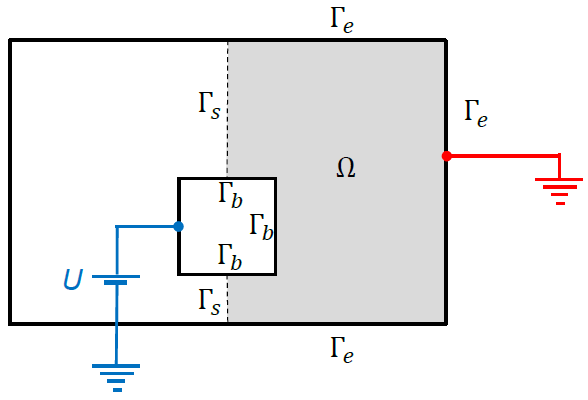
\includegraphics[width=8cm]{images/randbedinung_ES.png}
\end{minipage}
\subsection{Randwertproblem}
\begin{multicols}{2}
	\begin{itemize}
		\item $\dfrac{\partial^2\varphi}{\partial x^2} +  \dfrac{\partial^2\varphi}{\partial y^2} + \dfrac{\partial^2\varphi}{\partial z^2}=0 $
		\item $\varphi(x,y,z)=0 \in \Gamma_e$
		\item $\varphi(x,y,z)=U \in \Gamma_b$
		\item $ \dfrac{\partial\varphi(x,y,z)}{\partial r} = 0 \in \Gamma_s$
	\end{itemize}
\end{multicols}
\subsection{Vorgehen}
	\begin{enumerate}
		\item Partielle Differentialgleichung 2. Ordnung des Potentials aufstellen (Poisson oder Laplace)
		\item Koordinatentransformation wenn nötig
		\item Vereinfachung der partiellen DGL in eine gewöhnliche DGL 
		\subitem Von welcher Variable hängt das Potential ab
		\item Aufstellen der Randbedingungen
		\subitem Randwerte für Potential und E-Feld
		\item Gewöhnliche DGL 2x integrieren und nach Potential auflösen
		\item Randwerte einsetzen und unbekannte Konstanten bestimmen
	\end{enumerate}
\clearpage
\pagebreak